\chapter*{Campos de velocidades e de pressões para o problema de escoamento em torno de um cilindro.}
\addcontentsline{toc}{chapter}{APÊNDICE A}

\begin{figure}[h!]
    \centering
    \caption{Resultados no instante $t=120$ para elemento de aproximação linear.}
    \begin{subfigure}{\textwidth}
        \begin{subfigure}{\textwidth}\centering
            \begin{subfigure}{.42\textwidth}
                \caption*{Campo de velocidades.}
                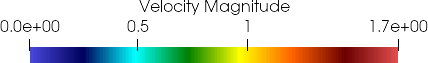
\includegraphics[width=\linewidth]{Figuras/cylinder/analise2/lu.png}
            \end{subfigure}
            \begin{subfigure}{.42\textwidth}
                \caption*{Campo de pressões.}
                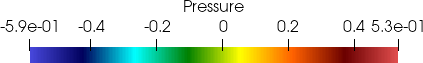
\includegraphics[width=\linewidth]{Figuras/cylinder/analise2/lp.png}
            \end{subfigure}
        \end{subfigure}
    \end{subfigure}
    \begin{subfigure}{\textwidth}\centering
        \begin{subfigure}{.49\textwidth}
            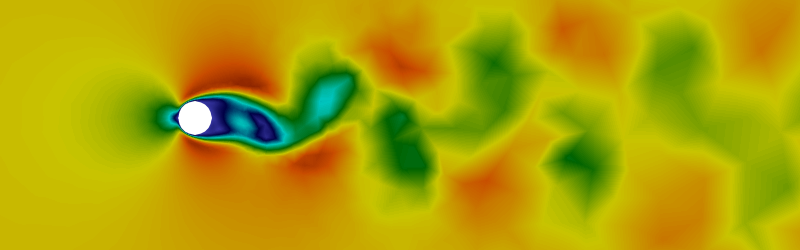
\includegraphics[width=\linewidth]{Figuras/cylinder/analise2/none-Lin-u.png}
        \end{subfigure}
        \begin{subfigure}{.49\textwidth}
            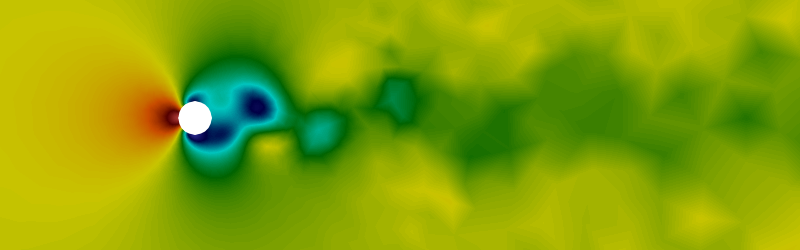
\includegraphics[width=\linewidth]{Figuras/cylinder/analise2/none-Lin-p.png}
        \end{subfigure}
        \caption{Sem modelo}
    \end{subfigure}
    \begin{subfigure}{\textwidth}\centering
        \begin{subfigure}{.49\textwidth}
            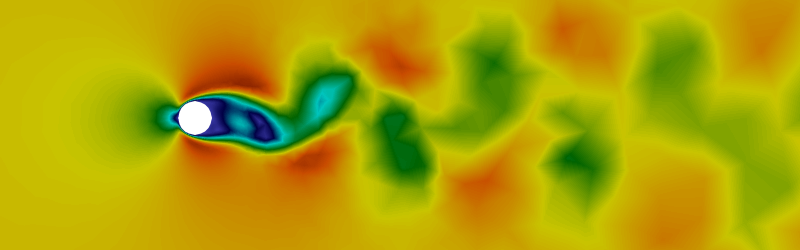
\includegraphics[width=\linewidth]{Figuras/cylinder/analise2/LES-Lin-u.png}
        \end{subfigure}
        \begin{subfigure}{.49\textwidth}
            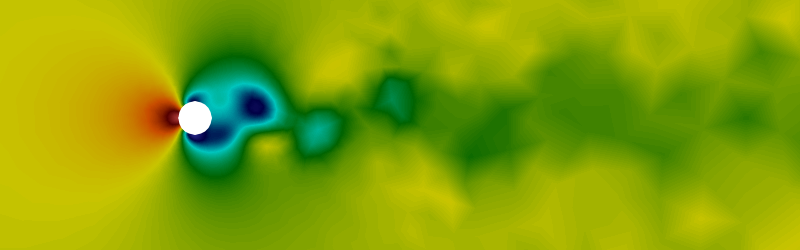
\includegraphics[width=\linewidth]{Figuras/cylinder/analise2/LES-Lin-p.png}
        \end{subfigure}
        \caption{LES}
    \end{subfigure}
    \begin{subfigure}{\textwidth}\centering
        \begin{subfigure}{.49\textwidth}
            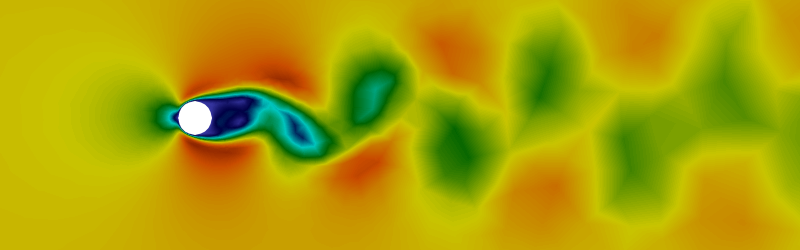
\includegraphics[width=\linewidth]{Figuras/cylinder/analise2/VMS-Lin-u.png}
        \end{subfigure}
        \begin{subfigure}{.49\textwidth}
            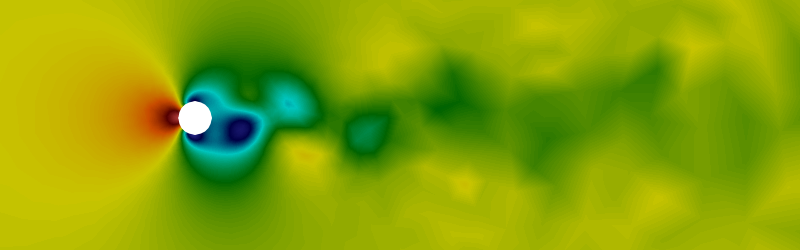
\includegraphics[width=\linewidth]{Figuras/cylinder/analise2/VMS-Lin-p.png}
        \end{subfigure}
        \caption{VMS}
    \end{subfigure}
    \\Fonte: Autoria Própria (\the\year).
\end{figure}

\begin{figure}[h!]
    \centering
    \caption{Resultados no instante $t=120$ para elemento de aproximação quadrática.}
    \begin{subfigure}{\textwidth}
        \begin{subfigure}{\textwidth}\centering
            \begin{subfigure}{.42\textwidth}
                \caption*{Campo de velocidades.}
                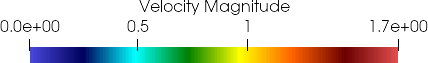
\includegraphics[width=\linewidth]{Figuras/cylinder/analise2/lu.png}
            \end{subfigure}
            \begin{subfigure}{.42\textwidth}
                \caption*{Campo de pressões.}
                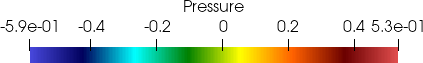
\includegraphics[width=\linewidth]{Figuras/cylinder/analise2/lp.png}
            \end{subfigure}
        \end{subfigure}
    \end{subfigure}
    \begin{subfigure}{\textwidth}\centering
        \begin{subfigure}{.49\textwidth}
            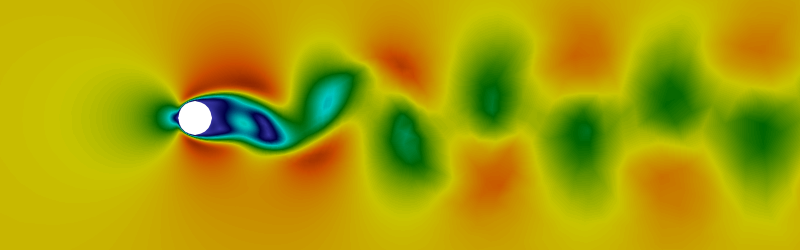
\includegraphics[width=\linewidth]{Figuras/cylinder/analise2/none-Qua-u.png}
        \end{subfigure}
        \begin{subfigure}{.49\textwidth}
            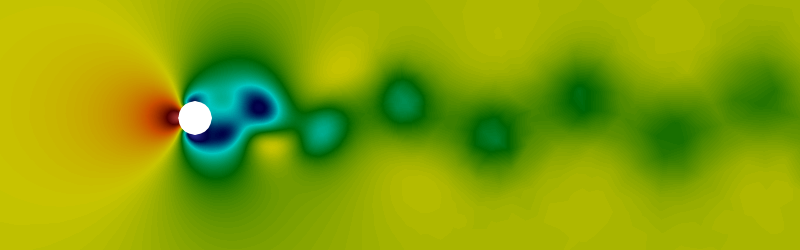
\includegraphics[width=\linewidth]{Figuras/cylinder/analise2/none-Qua-p.png}
        \end{subfigure}
        \caption{Sem modelo}
    \end{subfigure}
    \begin{subfigure}{\textwidth}\centering
        \begin{subfigure}{.49\textwidth}
            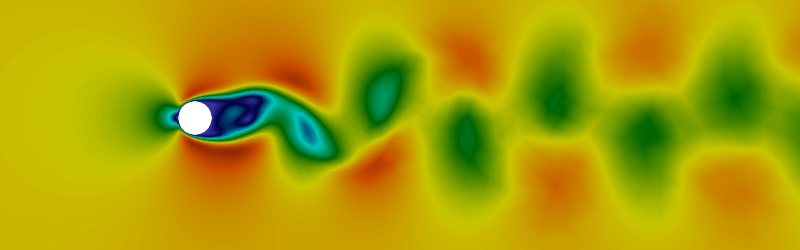
\includegraphics[width=\linewidth]{Figuras/cylinder/analise2/LES-Qua-u.png}
        \end{subfigure}
        \begin{subfigure}{.49\textwidth}
            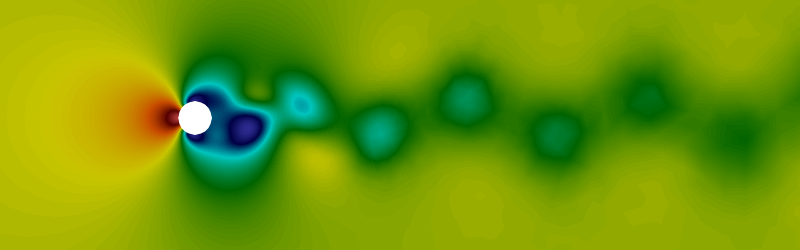
\includegraphics[width=\linewidth]{Figuras/cylinder/analise2/LES-Qua-p.png}
        \end{subfigure}
        \caption{LES}
    \end{subfigure}
    \begin{subfigure}{\textwidth}\centering
        \begin{subfigure}{.49\textwidth}
            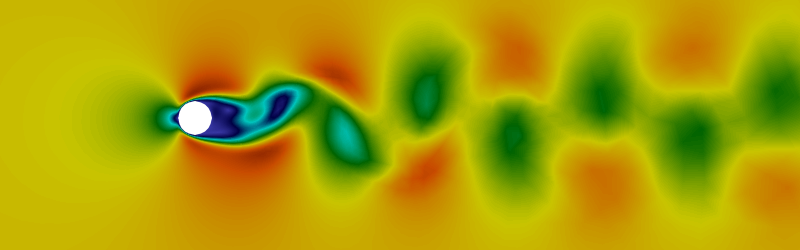
\includegraphics[width=\linewidth]{Figuras/cylinder/analise2/VMS-Qua-u.png}
        \end{subfigure}
        \begin{subfigure}{.49\textwidth}
            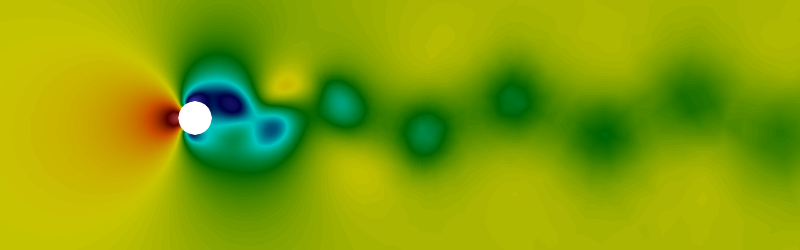
\includegraphics[width=\linewidth]{Figuras/cylinder/analise2/VMS-Qua-p.png}
        \end{subfigure}
        \caption{VMS}
    \end{subfigure}
    \\Fonte: Autoria Própria (\the\year).
\end{figure}

\begin{figure}[h!]
    \centering
    \caption{Resultados no instante $t=120$ para elemento Taylor-Hood P2P1.}
    \begin{subfigure}{\textwidth}
        \begin{subfigure}{\textwidth}\centering
            \begin{subfigure}{.42\textwidth}
                \caption*{Campo de velocidades.}
                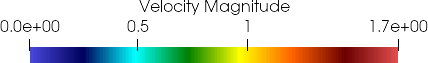
\includegraphics[width=\linewidth]{Figuras/cylinder/analise2/lu.png}
            \end{subfigure}
            \begin{subfigure}{.42\textwidth}
                \caption*{Campo de pressões.}
                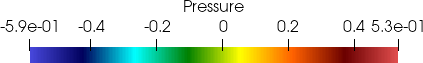
\includegraphics[width=\linewidth]{Figuras/cylinder/analise2/lp.png}
            \end{subfigure}
        \end{subfigure}
    \end{subfigure}
    \begin{subfigure}{\textwidth}\centering
        \begin{subfigure}{.49\textwidth}
            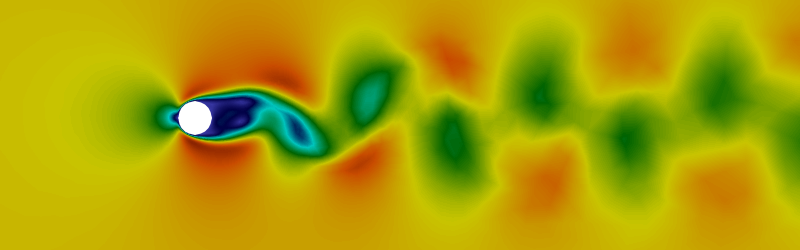
\includegraphics[width=\linewidth]{Figuras/cylinder/analise2/none-TH-u.png}
        \end{subfigure}
        \begin{subfigure}{.49\textwidth}
            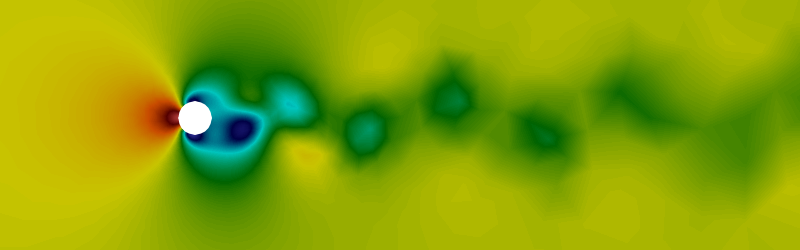
\includegraphics[width=\linewidth]{Figuras/cylinder/analise2/none-TH-p.png}
        \end{subfigure}
        \caption{Sem modelo}
    \end{subfigure}
    \begin{subfigure}{\textwidth}\centering
        \begin{subfigure}{.49\textwidth}
            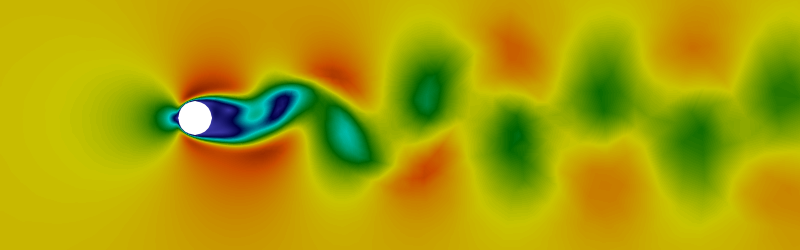
\includegraphics[width=\linewidth]{Figuras/cylinder/analise2/LES-TH-u.png}
        \end{subfigure}
        \begin{subfigure}{.49\textwidth}
            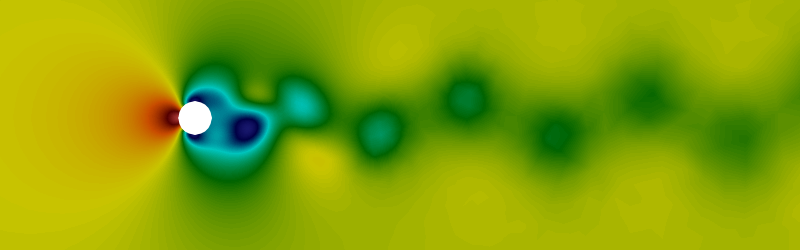
\includegraphics[width=\linewidth]{Figuras/cylinder/analise2/LES-TH-p.png}
        \end{subfigure}
        \caption{LES}
    \end{subfigure}
    \begin{subfigure}{\textwidth}\centering
        \begin{subfigure}{.49\textwidth}
            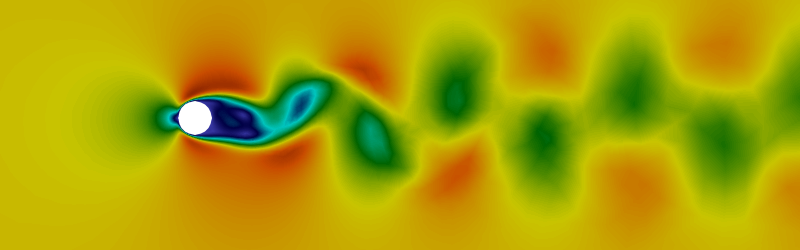
\includegraphics[width=\linewidth]{Figuras/cylinder/analise2/VMS-TH-u.png}
        \end{subfigure}
        \begin{subfigure}{.49\textwidth}
            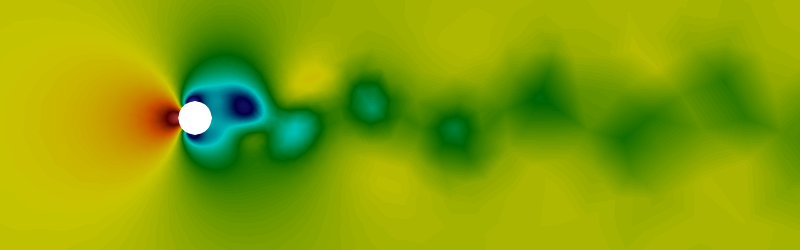
\includegraphics[width=\linewidth]{Figuras/cylinder/analise2/VMS-TH-p.png}
        \end{subfigure}
        \caption{VMS}
    \end{subfigure}
    \\Fonte: Autoria Própria (\the\year).
\end{figure}